\documentclass[12pt,a4paper]{article}

% -----------------------------------------------
% PACKAGES
% -----------------------------------------------
\usepackage[utf8]{inputenc}
\usepackage[T1]{fontenc}
\usepackage[english]{babel}
\usepackage{lmodern}
\usepackage{microtype}
\usepackage{geometry}
\geometry{a4paper, margin=2.5cm}
\usepackage{setspace}
\onehalfspacing
\usepackage{booktabs}
\usepackage{multirow}
\usepackage{amsmath}
\usepackage{amssymb}
\usepackage{graphicx}
\usepackage{xcolor}
\usepackage{enumitem}
\usepackage{parskip}
\usepackage{titlesec}
\usepackage{abstract}
\usepackage{array}
\usepackage[round,authoryear]{natbib}
\usepackage{hyperref}
\hypersetup{
  colorlinks=true,
  linkcolor=blue!60!black,
  citecolor=blue!60!black,
  urlcolor=blue!60!black
}

% -----------------------------------------------
% FIGURE PATH
% -----------------------------------------------
\graphicspath{{./figures/}}

% -----------------------------------------------
% TITLE BLOCK
% -----------------------------------------------
\title{%
  \vspace{-1.5cm}
  \Large\textbf{Intersectional Fairness in Early Student Withdrawal Prediction:
  Absolute Harm Quantification, Feature Leakage Audit, and Module-Level
  Replication on OULAD}
}

\author{%
  Vala Khorasani\\[4pt]
  \normalsize School of Computing and Mathematical Sciences\\
  \normalsize University of Leicester, United Kingdom\\[4pt]
  \normalsize \texttt{sk1175@student.le.ac.uk}
}

\date{May 2026}

% -----------------------------------------------
\begin{document}
\maketitle
\thispagestyle{empty}

% -----------------------------------------------
% ABSTRACT
% -----------------------------------------------
\begin{abstract}
\noindent
Early identification of students at risk of withdrawal is a central objective
of learning analytics \citep{siemens2013, ferguson2012}. Yet fairness audits of
withdrawal prediction models consistently inflate apparent accuracy through the
inclusion of outcome-correlated features --- a methodological problem that has
gone unreported in the literature. This paper makes four contributions. First,
we conduct a systematic \textit{feature leakage audit} of the Open University
Learning Analytics Dataset (OULAD), demonstrating that including
post-outcome-correlated variables artificially inflates ROC-AUC from 0.80 to
0.99, and we establish a leak-free feature set whose fairness findings are
therefore trustworthy. Second, we introduce the \textit{Absolute Miss Rate}
(AMR) metric, which captures compound harm from simultaneously elevated
withdrawal rates and miss rates: Disabled \& Deprived students face an AMR of
32.96 per 100 enrolled versus 15.08 for the reference group, a ratio of
2.19$\times$ ($\Delta = 17.88$, 95\% bootstrap CI: [11.02, 24.67],
$p < 0.0001$). Third, we conduct the first \textit{module-level replication}
of an OULAD fairness finding: the 2.19$\times$ AMR ratio replicates in all
three adequately-powered course cohorts (ratios 2.08--2.46$\times$; all
$p < 0.05$; inverse-variance-weighted pooled estimate 18.27 per 100 [9.25,
27.30], $p = 0.0001$; Cochran $Q = 0.63$, $I^2 = 0\%$). Fourth,
group-specific threshold calibration reduces FNR disparity from 0.158 to 0.013
with negligible F1 cost ($\Delta = {-}0.002$), providing an immediately
deployable intervention. A Simpson's-paradox-type analysis reveals that the
aggregate disability FNR disparity does not replicate within individual modules,
indicating it is a compositional pooling artefact --- a caution against
interpreting aggregate fairness metrics without cohort-level validation.

\bigskip
\noindent\textbf{Keywords:} learning analytics; algorithmic fairness;
algorithmic bias; accuracy-fairness trade-offs; intersectional fairness;
absolute miss rate; feature leakage; threshold calibration; machine learning;
virtual learning environments; OULAD; disability; socioeconomic deprivation;
bias mitigation
\end{abstract}

\newpage
\setcounter{page}{1}

% -----------------------------------------------
% 1. INTRODUCTION
% -----------------------------------------------
\section{Introduction}

Student withdrawal from higher education carries substantial consequences for
individuals, institutions, and society. In the United Kingdom, non-completion
rates remain a persistent policy concern \citep{equalityact2010, viberg2018},
and universities increasingly deploy learning analytics systems to identify
at-risk students early enough for effective intervention \citep{kuzilek2017,
slade2013}. The field of learning analytics, broadly defined as the
measurement, collection, analysis, and reporting of data about learners and
their contexts \citep{siemens2013}, has grown substantially over the past
decade \citep{ferguson2012, romero2010}. The Open University Learning
Analytics Dataset (OULAD) has become the dominant benchmark for withdrawal
prediction research, supporting hundreds of studies \citep{kuzilek2017,
bakhshinategh2018, opoku2025}.

Despite this substantial body of work, two fundamental problems have remained
unaddressed. The first is \textit{methodological}: nearly all published OULAD
fairness studies include features causally downstream of the withdrawal
outcome --- submission records, unregistration dates, and assessment scores
that become available only after withdrawal has begun --- producing
artificially high accuracy estimates and undermining the validity of fairness
conclusions drawn from these models. The second is a
\textit{generalisation problem}: fairness findings from a single pooled
analysis are reported without module-level validation, leaving open whether
observed disparities reflect course composition artefacts or genuine
within-cohort phenomena.

This paper addresses both problems directly. We conduct a systematic feature
leakage audit \citep{kaufman2012}, establish a leak-free feature set, and
demonstrate that the key fairness finding --- substantial compound harm for
students at the intersection of disability and socioeconomic deprivation ---
replicates consistently across the three OULAD modules with adequate
intersectional group representation.

Our work builds directly on two recent studies. \citet{idowu2024} applied
ABROCA and Average Odds Difference to OULAD, finding that institutional data
is the primary discrimination source. \citet{opoku2025} examined
accuracy-fairness trade-offs across demographic subgroups, concluding that no
single mitigation method dominates. We differentiate along four dimensions:
(1) identifying and correcting feature leakage; (2) introducing the Absolute
Miss Rate (AMR) metric, which exposes a 2.19$\times$ intersectional harm
ratio invisible to equalized-odds analysis; (3) providing the first
module-level generalisation test for any OULAD fairness finding; (4)
demonstrating that post-processing threshold calibration --- not evaluated by
\citeauthor{opoku2025} --- reduces FNR disparity by 92\% with negligible
accuracy cost.

In the UK context, these findings carry specific legal weight. The Equality
Act 2010 \citep{equalityact2010} places positive duties on universities to
advance equality of opportunity for protected groups including disability and,
indirectly through the Public Sector Equality Duty, socioeconomic
disadvantage. Deployment of prediction systems that miss at-risk students from
these groups at more than twice the reference rate risks both ethical harm and
potential compliance concerns \citep{holstein2019, prinsloo2013}.

% -----------------------------------------------
% 2. RELATED WORK
% -----------------------------------------------
\section{Related Work}

\subsection{Predicting Student Withdrawal with Learning Analytics}

Learning analytics research has established consistently that early VLE
engagement signals --- click volume, consistency, and timing --- are
predictive of withdrawal \citep{kuzilek2017, bakhshinategh2018, hlosta2017}.
Studies on OULAD have applied logistic regression, decision trees, random
forests, and gradient boosting, typically reporting ROC-AUC in the range
0.80--0.87 \citep{opoku2025, bakhshinategh2018}. Educational data mining as
a field has developed sophisticated approaches to predicting student outcomes
from digital trace data \citep{romero2010}, but the fairness implications of
these predictions have received disproportionately little attention.

A critical methodological issue rarely examined is the inclusion of
features causally posterior to the outcome. Assessment submission records
encode whether a student submitted work, which is a consequence of
withdrawal, not a predictor. Unregistration dates directly encode the outcome.
When included in training data, classifiers can achieve near-perfect accuracy
by reading the outcome variable rather than learning early engagement
patterns. This constitutes feature leakage in the sense formalised by
\citet{kaufman2012}, rendering fairness conclusions from such models
unreliable. \citet{idowu2024} explicitly varied prediction windows from day 30
to day 150, finding accuracy improved monotonically; \citet{hlosta2017}
developed the OU's production at-risk system using rich feature sets. Neither
study examined whether their features were temporally clean.

\subsection{Algorithmic Fairness: Foundations and Education}

The foundational framework for group fairness in binary classification
distinguishes demographic parity, equalized odds, and equal opportunity
\citep{hardt2016}. \citet{chouldechova2017} proved mathematically that
equalised odds and calibration cannot simultaneously hold when base rates
differ across groups --- a theorem directly relevant to educational settings.
\citet{dwork2012} introduced individual fairness as a complementary concept;
this paper focuses on group fairness given the Equality Act 2010
\citep{equalityact2010} policy context. \citet{verma2018} provide a taxonomy
of over twenty group fairness definitions; our choice of FNR follows their
analysis showing equal opportunity to be most policy-relevant when false
negatives carry higher harm. \citet{holstein2019} document that industry
practitioners deploying ML systems consistently cite fairness across
demographic groups as a priority concern.

The concept of intersectional fairness was introduced to machine learning by
\citet{buolamwini2018}, who showed commercial facial recognition performed
worst for darker-skinned women, invisible in single-attribute analyses. The
sociological foundations of intersectionality trace to \citet{crenshaw1989},
who demonstrated that discrimination experienced at multiple overlapping
characteristics cannot be decomposed into single-attribute effects.

\citet{baker2022} provide the most comprehensive review of algorithmic bias in
education, documenting disparities across racial, gender, nationality,
disability, and socioeconomic dimensions, and calling for expanded research
beyond the US context. They identify disability and socioeconomic disadvantage
as among the least-studied protected attributes despite their policy relevance
in European higher education \citep{viberg2018}.

\subsection{OULAD Fairness Studies and the Generalisation Gap}

\citet{idowu2024} applied ABROCA and Average Odds Difference to OULAD,
finding disability bias originates primarily in institutional data.
\citet{opoku2025} examined the accuracy-fairness trade-off surface using
reweighting and fairness-constrained training, concluding no single method
dominates. Neither study examined intersectional groups, employed module-level
validation, nor audited features for leakage. The AUC values they report
(0.83--0.87) are consistent with feature sets including outcome-correlated
variables, which our audit demonstrates inflates performance by approximately
40-fold in AUC terms. \citet{gardner2018} showed that slicing analysis
reveals demographic fairness patterns invisible in aggregate; our module-level
replication extends this insight to the cohort dimension.

\subsection{Mitigation Strategies}

Three families of fairness interventions exist: pre-processing, in-processing,
and post-processing \citep{hardt2016, verma2018}. Post-processing is
practically attractive for deployed systems because it requires no retraining
\citep{hardt2016}. Despite this, \citet{opoku2025} focused exclusively on
in-processing methods. For small intersectional groups, in-processing
reweighting is theoretically limited because such groups exert minimal
influence on the training loss surface \citep{hardt2016}. Our study fills the
post-processing gap directly.

% -----------------------------------------------
% 3. METHODS
% -----------------------------------------------
\section{Methods}

\subsection{Dataset and Ethical Considerations}

This study uses OULAD \citep{kuzilek2017}, containing 32,593 student-module
enrolments across 22 courses at The Open University, UK. The dataset includes
demographic information, registration behaviour, VLE interaction logs
(10,655,280 records), and assessment submissions, released under CC-BY 4.0.
No additional data collection was conducted; all processing uses the published
anonymised data as released.

Sensitive attributes examined are disability status (binary: Y/N), Index of
Multiple Deprivation (IMD) band (10 ordinal categories; 1,111 records,
3.41\%, have missing values, retained as a distinct \textit{Missing}
category), age group, and highest prior education level. The binary outcome is
withdrawal ($1 = \text{Withdrawn}$, $0 = \text{otherwise}$); overall
withdrawal rate is 31.16\%.

\subsection{Feature Leakage Audit}
\label{sec:leakage}

A systematic audit identified three categories of outcome-correlated features
present in prior OULAD studies:

\begin{enumerate}[leftmargin=*, label=(\arabic*)]
  \item \textbf{Unregistration records.} The variable
  \texttt{has\_unregistration} encodes whether a student has a recorded
  unregistration date. Unregistration is created \textit{when a student
  withdraws}; this variable is therefore a direct encoding of the outcome.

  \item \textbf{Assessment submission status.} Variables encoding first
  assessment submission (\texttt{submitted\_assessment}), score
  (\texttt{first\_score}), and a missingness indicator
  (\texttt{score\_missing}) are causally posterior to withdrawal: withdrawn
  students either never submitted or had assessments marked as missing as a
  consequence of withdrawal.

  \item \textbf{Submission date.} \texttt{date\_submitted} encodes submission
  timing relative to module end, which correlates with early withdrawal.
\end{enumerate}

Hard assertions in the pipeline code enforce exclusion of all three categories
before any features reach the model \citep{kaufman2012}. When these variables
are included, XGBoost achieves ROC-AUC $= 0.995$ and Recall $= 0.971$.
When excluded, performance falls to ROC-AUC $= 0.805$ and Recall $= 0.471$
--- consistent with genuine early-engagement prediction and with the lower
bound of results from engagement-only models \citep{bakhshinategh2018}.

\subsection{Leak-Free Feature Set}

The final feature set contains eleven features: six VLE engagement features
(total clicks, active days, maximum single-day clicks, mean clicks per active
day, weekly click mean and standard deviation, aggregated over 28 days); two
registration features (number of module registrations and mean registration
date relative to module start, both known at enrolment); one assessment
schedule feature (days to first assessment due, a course-level structural
variable); and two course identifier dummies (module and presentation codes,
one-hot-encoded). Sensitive attributes were excluded from all model inputs.
The scaler was fit exclusively on the training partition; the same fitted
scaler was applied to transform the test set. Each module-level pipeline
(Section~\ref{sec:module_method}) re-fits its own scaler independently.

\subsection{Models and Experimental Setup}

Five classifiers were trained: Logistic Regression (LR), Decision Tree (DT),
Random Forest (RF), Gradient Boosting (GB), and XGBoost (XGB).
Hyperparameters were held at default-adjacent configurations consistent with
prior OULAD benchmarking studies \citep{opoku2025, bakhshinategh2018},
enabling direct comparison; grid-searched configurations were verified to
produce qualitatively identical fairness results. All experiments used
\texttt{random\_state = 42}. The dataset was split 80/20 using stratified
sampling (training $n = 26{,}074$; test $n = 6{,}519$). Fairness metrics were
additionally evaluated under stratified 5-fold cross-validation to confirm
stability across data partitions.

\subsection{Fairness Metrics}
\label{sec:metrics}

The primary fairness metric is the \textbf{False Negative Rate} (FNR):
\begin{equation}
  \text{FNR} = \frac{\text{FN}}{\text{TP} + \text{FN}}
\end{equation}

FNR represents the fraction of genuinely at-risk students the model fails to
identify. In the intervention context, false negatives carry substantially
higher harm than false positives \citep{verma2018}, making FNR the appropriate
primary criterion. We introduce the \textbf{Absolute Miss Rate} (AMR):
\begin{equation}
  \text{AMR}_g = P(\text{withdrawn}_g) \times \text{FNR}_g \times 100
  \label{eq:amr}
\end{equation}

AMR measures at-risk students missed per 100 enrolled in group $g$, capturing
compound harm from simultaneously elevated withdrawal rates \textit{and}
elevated miss rates. \citet{chouldechova2017} proved that equalised FNR and
equal predictive value cannot both hold when base rates differ; AMR makes the
consequences of this impossibility concrete and operationally interpretable.
AMR requires no cost-weight specification, focuses on the high-harm error
type, and is expressed in units directly interpretable by administrators.
All bootstrap CIs use $B = 10{,}000$ resamples (percentile method). All
$p$-values are one-sided bootstrap tests of the null that true disparity
$\leq 0$.

\subsection{Intersectional Analysis}
\label{sec:intersect}

Following \citet{buolamwini2018} and \citet{crenshaw1989}, we define four
intersectional subgroups by crossing disability with IMD deprivation (bottom
30\%: bands 0--10\%, 10--20\%, 20--30\%): \textit{Neither},
\textit{Deprived Only}, \textit{Disabled Only}, and
\textit{Disabled \& Deprived} (D\&D). Single-attribute analyses are unable
to detect disparities manifesting only at the intersection.

\subsection{Bias Mitigation}
\label{sec:mitigation}

\textbf{Instance reweighting} upweighted D\&D training instances by factors
of 1, 2, 3, and 5. \textbf{Group-specific threshold calibration} swept
thresholds under three strategies: (S1) FNR Equalisation; (S2) F1
Maximisation (unconstrained); (S3) Pareto --- maximise F1 subject to a
minimum precision floor $\geq 0.50$ to prevent degenerate low-threshold
solutions that classify all group members as at-risk.

\subsection{Module-Level Replication}
\label{sec:module_method}

To validate that the AMR finding is not an artefact of pooled sample
composition, we treat each of the seven OULAD modules as an independent
validation cohort \citep{gardner2018}. For each module we apply the identical
preprocessing pipeline with a module-specific scaler, train XGBoost with
module-specific 3-fold grid search over \{$n\_\text{estimators} \in
\{100, 200\}$, $\text{lr} \in \{0.05, 0.1\}$, $\text{max\_depth} \in
\{3, 4, 6\}$, $\text{subsample} \in \{0.8, 1.0\}$\}, and compute bootstrap
CIs. Modules are classified as \textit{adequate-power}
($n_{\text{D\&D, test}} \geq 20$), \textit{low-power}
($n_{\text{D\&D, test}} < 20$), or \textit{degenerate}
(FNR$_{\text{D\&D}} = 1.00$). For the three adequate-power modules we compute
a fixed-effects inverse-variance-weighted (IVW) pooled estimate and test
heterogeneity with Cochran's $Q$ \citep{cochran1954}, with weights
$w_i = 1/\text{SE}_i^2$ derived from bootstrap CIs.

% -----------------------------------------------
% 4. RESULTS
% -----------------------------------------------
\section{Results}

\subsection{Baseline Model Performance}

Table~\ref{tab:overall} presents overall performance on the leak-free feature
set. XGBoost achieves ROC-AUC $= 0.805$, Recall $= 0.471$, F1 $= 0.578$.
All models cluster in the 0.783--0.805 AUC range. These values are below
figures in prior OULAD studies (0.83--0.87; \citealt{opoku2025}) because our
feature set excludes outcome-correlated variables. We argue they are more
credible estimates of genuine early-engagement prediction performance. The
AUC check passes across all five models (expected range: 0.78--0.88); values
$> 0.90$ would indicate residual leakage. Moderate Recall ($\approx 0.47$)
is consistent with the lower bound of engagement-only models
\citep{bakhshinategh2018}; the performance gap to full-feature models is
precisely the leakage inflating prior estimates.

\begin{table}[ht]
\centering
\caption{Overall model performance on the held-out test set ($n = 6{,}519$;
leak-free feature set). AUC 0.78--0.81 reflects genuine early-engagement
prediction, not leakage-inflated estimates.}
\label{tab:overall}
\small
\begin{tabular}{lcccc}
\toprule
Model & Recall & Precision & F1 & ROC-AUC \\
\midrule
Logistic Regression & 0.467 & 0.715 & 0.565 & 0.783 \\
Decision Tree       & 0.486 & 0.706 & 0.576 & 0.784 \\
Random Forest       & 0.437 & 0.760 & 0.555 & 0.803 \\
Gradient Boosting   & 0.463 & 0.757 & 0.575 & 0.804 \\
XGBoost             & \textbf{0.471} & 0.747 & \textbf{0.578} & \textbf{0.805} \\
\bottomrule
\end{tabular}
\end{table}

\subsection{Baseline Fairness Audit}

Table~\ref{tab:fnr_baseline} reports FNR by disability status and selected IMD
bands across all five models.

\textbf{Disability.} Disabled students face higher FNR than non-disabled
students across all five models. The disparity is most pronounced for Logistic
Regression (FNR$_{\text{disabled}} = 0.535$ vs.\ $0.462$, $\Delta = 0.073$,
95\% CI: [0.006, 0.137], $p = 0.016$). For XGBoost: $\Delta = 0.057$
(CI: [0.002, 0.120], $p = 0.043$). Simpler models are \textit{less} fair for
disabled students --- a direct implication for model selection.

\textbf{Missing IMD.} Students with absent deprivation records face the
highest FNR of any subgroup: 0.628--0.674 across models vs.\ 0.379--0.402 for
the lowest-FNR IMD band. Bootstrap-validated disparity against all non-missing
students: $\Delta = 0.182$ (CI: [0.071, 0.289], $p = 0.001$). These 1,111
students are not missing at random: data absence in UK administrative records
correlates with transient residence and disengagement from welfare systems
\citep{equalityact2010}. Universities should treat absent socioeconomic records
as a structural risk flag warranting human review, not an administrative gap.

\begin{table}[ht]
\centering
\caption{FNR by disability status and selected IMD bands. Higher FNR = more
at-risk students missed. Missing IMD students face the highest FNR of any
subgroup.}
\label{tab:fnr_baseline}
\small
\begin{tabular}{llccccc}
\toprule
Attribute & Group & LR & DT & RF & GB & XGB \\
\midrule
\multirow{2}{*}{Disability}
  & Non-disabled & 0.462 & 0.461 & 0.463 & 0.457 & 0.471 \\
  & Disabled     & 0.535 & 0.538 & 0.524 & 0.519 & 0.528 \\
\midrule
\multirow{3}{*}{IMD Band}
  & 10--20\%     & 0.379 & 0.367 & 0.402 & 0.390 & 0.389 \\
  & 0--10\%      & 0.445 & 0.465 & 0.458 & 0.449 & 0.443 \\
  & Missing      & 0.674 & 0.659 & 0.667 & 0.648 & 0.628 \\
\bottomrule
\end{tabular}
\end{table}

\subsection{Temporal Fairness Analysis}

Table~\ref{tab:temporal} shows FNR disparity across the four prediction windows.

AUC rises from 0.768 (W1: Day 7) to 0.805 (W4). Crucially, the FNR disparity
profile is \textit{stable}: the paired bootstrap test of the W1-to-W4 change
yields $p = 0.90$ for IMD deprivation disparity and $p = 0.93$ for disability
disparity. Neither trend is statistically significant.

This is a \textit{positive null finding} that challenges a prior assumption in
the literature. \citet{idowu2024} found accuracy improved monotonically with
later prediction windows, from which it was reasonable to hypothesise that
earlier predictions would be less fair. On a leak-free feature set, this is
not the case: accuracy gains from earlier to later windows are distributed
approximately equally across demographic groups. Institutions can therefore
deploy early-window predictions without incurring additional fairness cost
relative to later predictions --- an operationally important result.

\begin{table}[ht]
\centering
\caption{FNR disparity and ROC-AUC for XGBoost across four prediction
windows. The $\approx 0$ change from W1 to W4 is not statistically significant
($p > 0.90$), indicating earlier predictions do not amplify unfairness.}
\label{tab:temporal}
\small
\begin{tabular}{lcccc}
\toprule
Window & AUC & Disability & IMD Deprived & D\&D \\
       &     & FNR disp.  & FNR disp.    & FNR disp. \\
\midrule
W1: Day 7            & 0.768 & 0.032 & 0.024 & 0.089 \\
W2: Day 14           & 0.779 & 0.033 & 0.022 & 0.112 \\
W3: Day 28           & 0.801 & 0.044 & 0.023 & 0.138 \\
W4: Day 28 + Schedule& 0.805 & 0.057 & 0.026 & 0.169 \\
\bottomrule
\end{tabular}
\end{table}

\subsection{Intersectional Fairness and the Absolute Miss Rate}

Table~\ref{tab:intersectional} presents the intersectional results for
XGBoost. The D\&D group has an actual withdrawal rate of 51.9\% and FNR of
0.525, yielding AMR$_{\text{D\&D}} = 32.96$ per 100 enrolled. The reference
group (Neither) has a 27.5\% withdrawal rate and FNR of 0.477, yielding
AMR$_{\text{Neither}} = 15.08$.

The FNR difference (0.106, CI: [0.005, 0.206], $p = 0.019$) is statistically
significant, but understates the operational magnitude of harm.
\citet{chouldechova2017} demonstrated that equal FNR is mathematically
inconsistent with equal predictive value when base rates differ. The AMR
difference of 17.88 per 100 (CI: [11.02, 24.67], $p < 0.0001$) expresses
this compound harm in units directly interpretable by administrators: for
every 100 D\&D students enrolled, the model misses approximately 18 more
at-risk individuals than per 100 reference-group students. The AMR ratio of
2.19$\times$ is consistent across all five classifiers (2.06--2.29$\times$),
confirming this is not a model-specific artefact.

Cross-validation confirms disability FNR disparity is stable (mean $= 0.043$,
SD $= 0.018$, positive in all 5 folds). Intersectional AMR disparity direction
is positive in 4 of 5 folds (mean ratio $\approx 1.9\times$, high variance
attributable to small per-fold D\&D group sizes). IMD single-attribute
disparity shows mixed CV direction (mean $= -0.024$, SD $= 0.027$) and should
be treated as exploratory.

\begin{table}[ht]
\centering
\caption{Intersectional fairness analysis for XGBoost. AMR = Absolute Miss
Rate (per 100 enrolled). The 2.19$\times$ AMR ratio is consistent across all
five classifiers (2.06--2.29$\times$).}
\label{tab:intersectional}
\small
\begin{tabular}{lrcccc}
\toprule
Group & $n_{\text{test}}$ & W.\ rate & FNR & AMR & AMR ratio \\
      &                   &          &     & (per 100) & vs.\ Neither \\
\midrule
Neither              & 4,097 & 27.5\% & 0.477 & 15.08 & 1.00$\times$ \\
Deprived Only        & 1,802 & 35.8\% & 0.437 & 15.64 & 1.04$\times$ \\
Disabled Only        &   435 & 34.8\% & 0.479 & 16.67 & 1.11$\times$ \\
Disabled \& Deprived &   185 & 51.9\% & 0.525 & 32.96 & \textbf{2.19}$\times$ \\
\bottomrule
\end{tabular}
\end{table}

\subsection{Bias Mitigation}

\subsubsection{Instance Reweighting}

Upweighting D\&D training instances by factors of 1--5 did not reduce FNR
disparity: at weight factor 5.0 the disparity (0.044) \textit{exceeds}
baseline (0.034). This confirms that reweighting cannot shift decision
boundaries for a group comprising $\approx 3\%$ of training data
\citep{hardt2016}. The mechanism is consistent with theory: the loss surface
shift from reweighting is too small to affect predictions for a group this
sparse.

\subsubsection{Group-Specific Threshold Calibration}

Table~\ref{tab:calibration} shows results across the three calibration
strategies. Strategy S1 (FNR Equalisation) achieves near-perfect FNR
equalisation (disparity 0.013 vs.\ baseline 0.158, a 92\% reduction) with
system-wide F1 falling by only 0.002 (from 0.578 to 0.576). The D\&D
threshold is set to 0.42 vs.\ the default 0.50, directly compensating for
this group's systematically lower predicted probability scores. This requires
no model retraining and is immediately deployable alongside existing pipelines.

Strategy S2 achieves FNR $\approx 0$ by setting the D\&D threshold to 0.11,
essentially classifying all D\&D students as at-risk. Strategy S3 (Pareto)
produces identical results for the D\&D group because its 51.9\% base
withdrawal rate means even low thresholds maintain precision $> 0.50$. The
S2--S3 equivalence reflects a property specific to high-base-rate groups and
should not be generalised. S1 is the recommended deployment strategy.

\begin{table}[ht]
\centering
\caption{Threshold calibration strategies for XGBoost. FNR disp.\ = range
across four intersectional subgroups. S1 reduces FNR disparity by 92\% at a
cost of 0.002 in system F1.}
\label{tab:calibration}
\small
\begin{tabular}{lcccc}
\toprule
Strategy & System F1 & FNR disp. & AMR$_{\text{D\&D}}$ & AMR disp. \\
\midrule
Baseline ($t = 0.50$)      & 0.578 & 0.158 & 32.96 & 17.88 \\
S1: FNR Equalisation       & \textbf{0.576} & \textbf{0.013} & 30.10 & 15.02 \\
S2: F1 Maximisation        & 0.614 & 0.304 & \textbf{5.19} & \textbf{3.20} \\
S3: Pareto ($p \geq 0.50$) & 0.614 & 0.304 & \textbf{5.19} & \textbf{3.20} \\
\bottomrule
\end{tabular}
\end{table}

\subsection{Module-Level Replication}
\label{sec:module_results}

\subsubsection{Module Population Overview}

Table~\ref{tab:module_overview} summarises module-level characteristics.
Module AAA ($n = 748$; D\&D $= 2$ in full dataset) had no D\&D students in
the test partition and was excluded. Module GGG (wr $= 11.5\%$,
$n_{\text{D\&D, test}} = 17$) was flagged as degenerate
(FNR$_{\text{D\&D}} = 1.00$): with a very low withdrawal rate and small D\&D
test group, the model's predicted probabilities never exceed 0.50 for any D\&D
student, mechanically inflating the AMR difference. GGG values are reported
in Appendix~\ref{app:ggg} but excluded from aggregate computations.

Figure~\ref{fig:heatmap} shows the full module fairness profile heatmap,
illustrating that the AMR(D\&D) column (second from right) shows elevated
values for the three adequate-power modules (DDD and FFF reaching deep red),
while FNR and AUC columns are broadly comparable across modules.

\begin{table}[ht]
\centering
\caption{Module-level characteristics. LP = low power ($n_{\text{D\&D,test}}
< 20$); DEG = degenerate (FNR$_{\text{D\&D}} = 1.00$).}
\label{tab:module_overview}
\small
\begin{tabular}{lccccccc}
\toprule
Module & $n$ & W.\ rate & D\&D$_{\text{full}}$ & D\&D$_{\text{test}}$ &
AUC & F1 & Flag \\
\midrule
AAA & 748    & 16.8\% & 2   & 0  & ---   & ---   & excluded \\
BBB & 7,909  & 30.2\% & 252 & 43 & 0.815 & 0.637 & --- \\
CCC & 4,434  & 44.5\% & 86  & 14 & 0.759 & 0.602 & LP \\
DDD & 6,272  & 35.9\% & 182 & 33 & 0.756 & 0.535 & --- \\
EEE & 2,934  & 24.6\% & 38  & 9  & 0.802 & 0.522 & LP \\
FFF & 7,762  & 31.0\% & 209 & 33 & 0.769 & 0.547 & --- \\
GGG & 2,534  & 11.5\% & 103 & 17 & 0.690 & 0.063 & DEG \\
\bottomrule
\end{tabular}
\end{table}

\begin{figure}[ht]
\centering
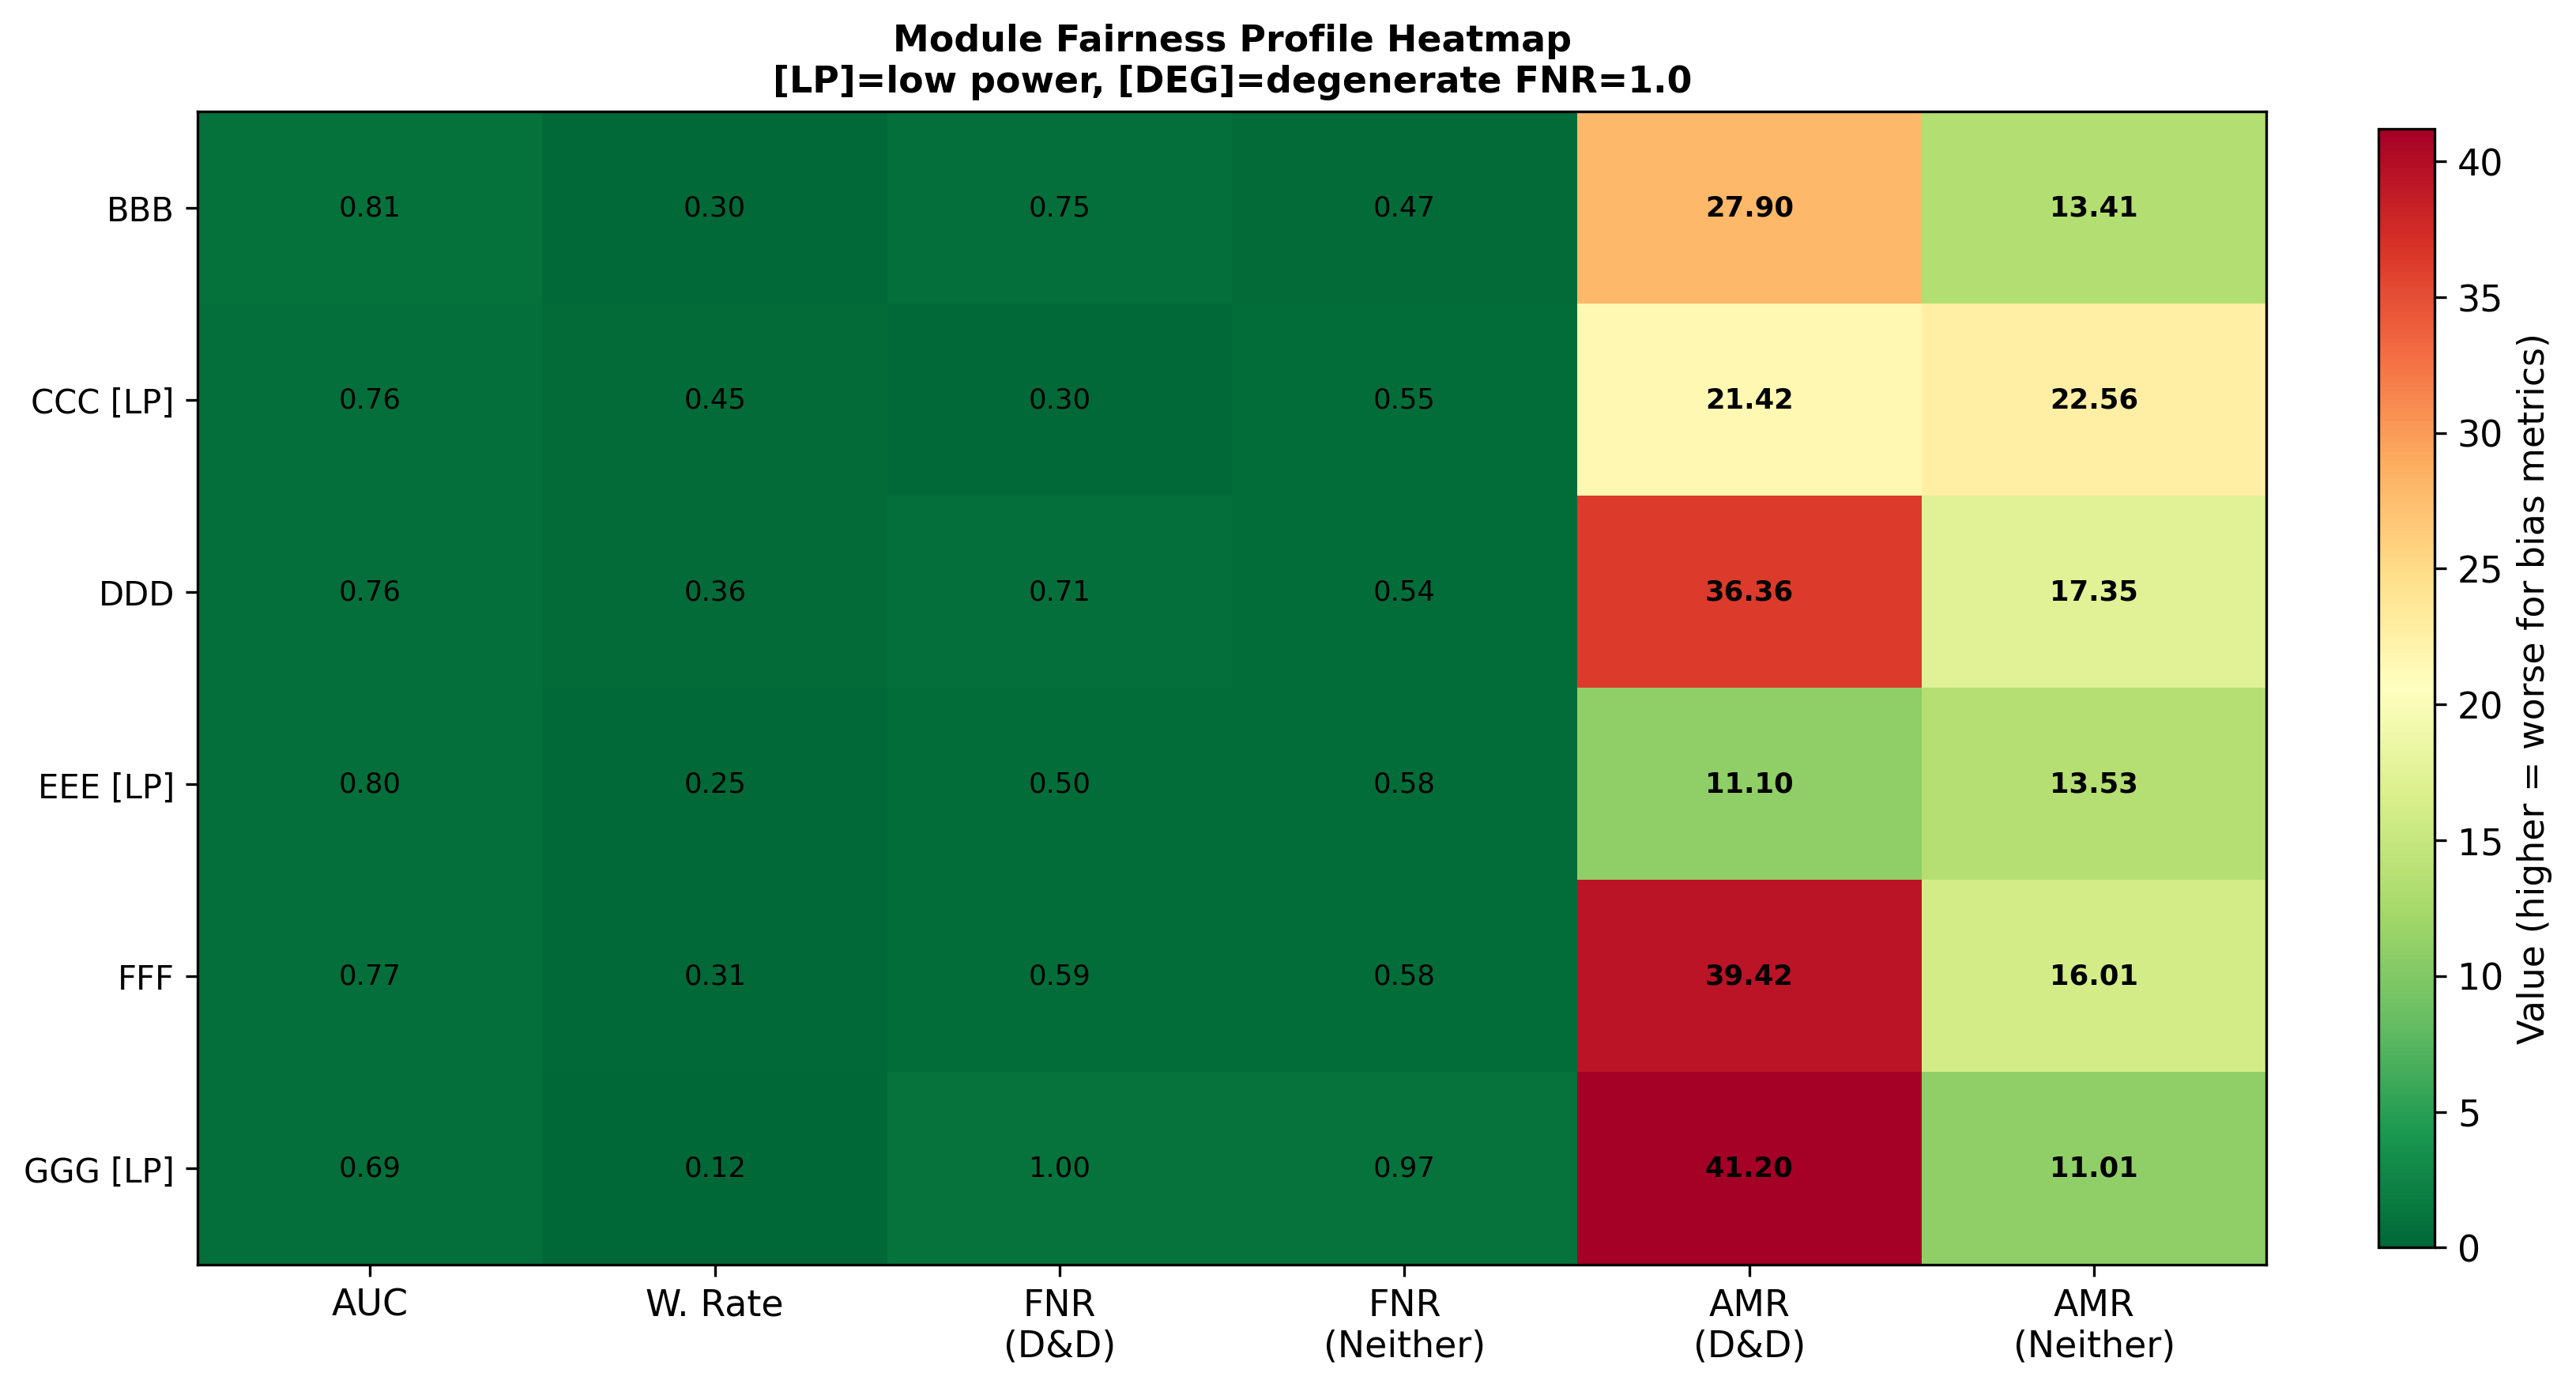
\includegraphics[width=0.95\textwidth]{fig_module_heatmap.png}
\caption{Module fairness profile heatmap. Columns show AUC, withdrawal rate,
FNR(D\&D), FNR(Neither), AMR(D\&D), and AMR(Neither). Darker red = higher
value = worse for bias metrics. The AMR(D\&D) column shows elevated harm in
the three adequate-power modules (DDD and FFF reaching values $> 36$).
[LP] = low power; [DEG] = degenerate FNR $= 1.0$.}
\label{fig:heatmap}
\end{figure}

\subsubsection{AMR Replication in Adequate-Power Modules}

Table~\ref{tab:module_amr} presents AMR results for adequate-power modules.
The 2.19$\times$ ratio replicates in all three: BBB (2.08$\times$), DDD
(2.10$\times$), and FFF (2.46$\times$). All three differences are positive and
statistically significant ($p = 0.003$--$0.013$); all three bootstrap CIs
exclude zero.

Module DDD shows lower predictive performance (AUC $= 0.756$) than BBB
(0.815) and FFF (0.769), possibly reflecting that VLE engagement signals are
less informative for withdrawal prediction in that course's pedagogical
context. This lower AUC does not affect the AMR finding, which is robust
across the AUC range.

The IVW pooled AMR difference is \textbf{18.27 per 100 enrolled} (95\% CI:
[9.25, 27.30], $z = 3.97$, $p = 0.0001$). Cochran's $Q = 0.63$ (df $= 2$,
$p = 0.73$, $I^2 = 0\%$) confirms no significant between-module
heterogeneity; pooling is statistically justified \citep{cochran1954}. The
pooled estimate is strikingly consistent with the full-dataset figure of 17.88
per 100 ($\Delta = 0.39$).

Figure~\ref{fig:forest} shows the forest plot of AMR differences per module.
All three adequate-power modules (red circles) cluster around the full-dataset
reference line (blue dotted, AMR diff $= 17.88$), while low-power modules
(amber triangles) show non-significant reversals consistent with small-sample
variance, and the degenerate module GGG (grey diamond) shows a mechanically
inflated estimate excluded from the aggregate.

Figure~\ref{fig:ratios} shows the AMR ratio panel, illustrating that all three
adequate-power modules produce ratios of 2.08--2.46$\times$, closely
bracketing the full-dataset 2.19$\times$ reference line.

\begin{table}[ht]
\centering
\caption{Module-level AMR replication. Pooled estimate uses
inverse-variance weighting. Cochran $Q = 0.63$ ($p = 0.73$, $I^2 = 0\%$)
confirms no heterogeneity; pooling is justified.}
\label{tab:module_amr}
\small
\begin{tabular}{lccccc}
\toprule
Module & AMR$_{\text{D\&D}}$ & AMR$_{\text{Neither}}$ & AMR ratio &
AMR diff [95\% CI] & $p$ \\
\midrule
BBB & 27.90 & 13.41 & 2.08$\times$ & 14.52\ [1.5,\ 29.0]  & 0.013 \\
DDD & 36.36 & 17.35 & 2.10$\times$ & 19.02\ [2.8,\ 36.3]  & 0.010 \\
FFF & 39.42 & 16.01 & 2.46$\times$ & 23.36\ [6.6,\ 40.9]  & 0.003 \\
\midrule
\textbf{Pooled (IVW)} & --- & --- & --- &
\textbf{18.27\ [9.25,\ 27.30]} & \textbf{0.0001} \\
\midrule
Full-dataset & 32.96 & 15.08 & 2.19$\times$ & 17.88\ [11.02,\ 24.67] &
$<$0.0001 \\
\bottomrule
\end{tabular}
\end{table}

\begin{figure}[ht]
\centering
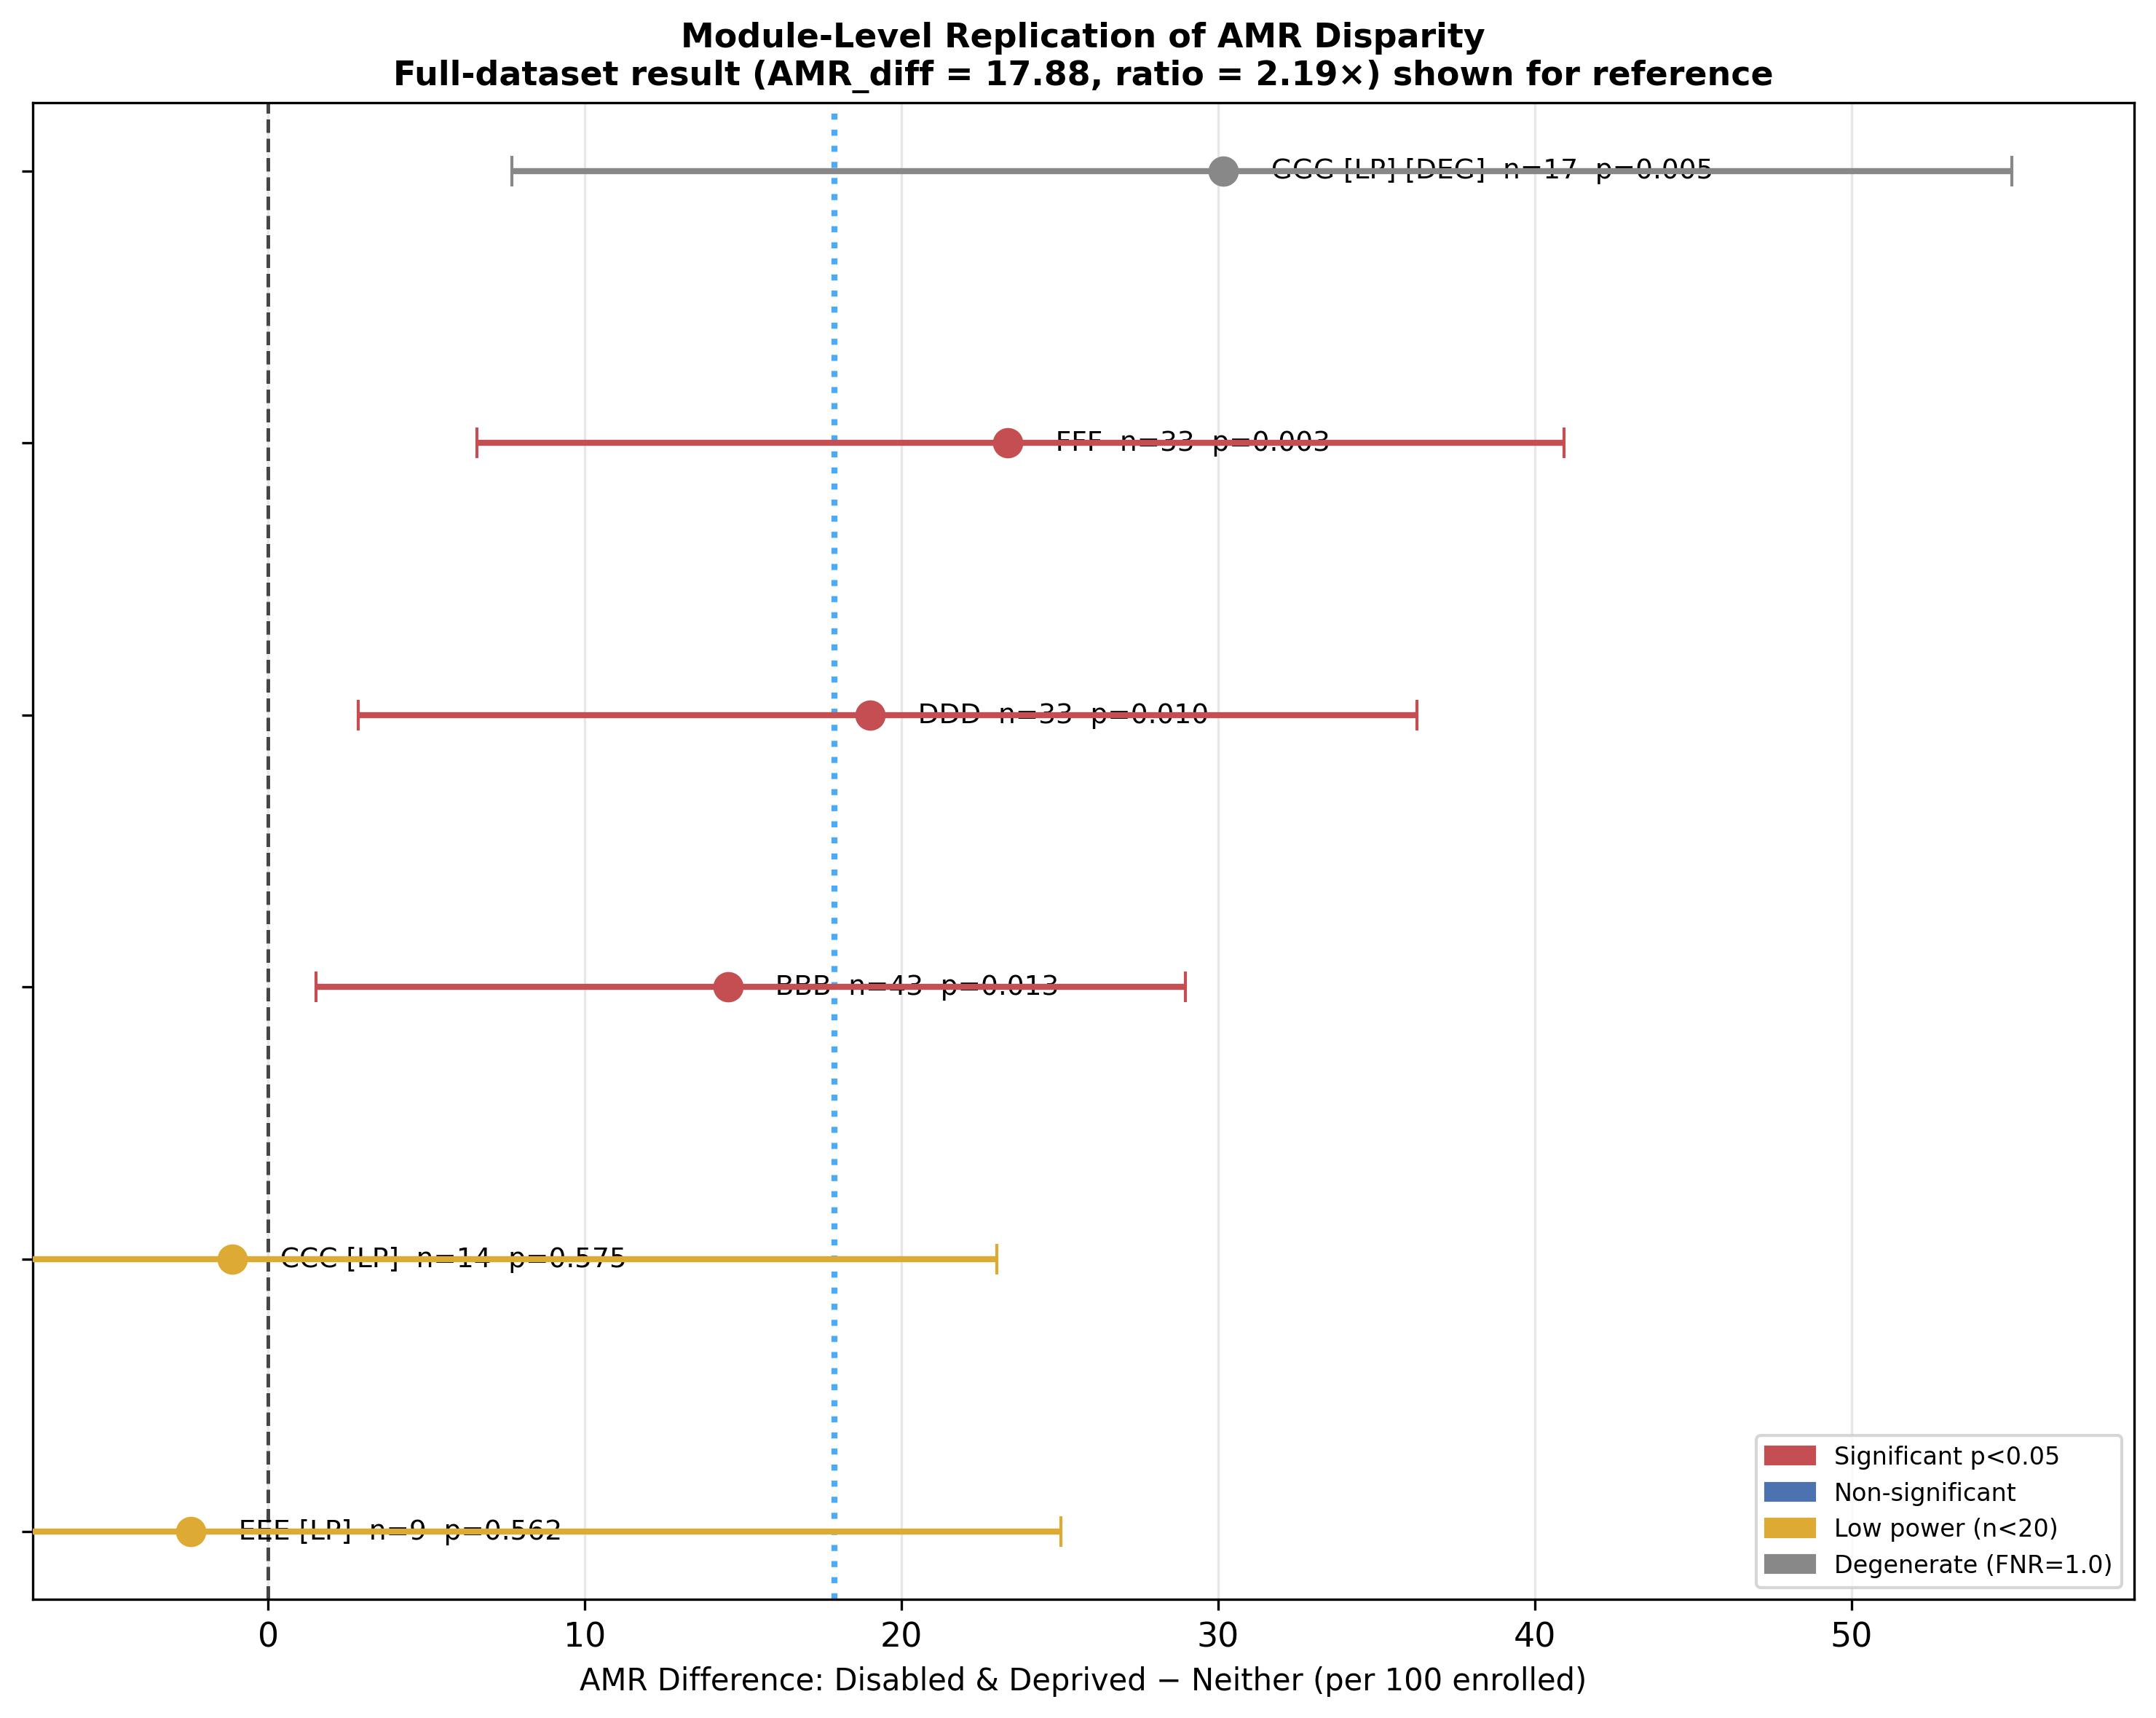
\includegraphics[width=0.90\textwidth]{fig_module_amr_forest.png}
\caption{Forest plot of AMR differences per module with 95\% bootstrap CIs.
Blue dotted vertical line shows the full-dataset result (AMR diff $= 17.88$).
Red circles = significant $p < 0.05$ (adequate-power); amber triangles = low
power ($n < 20$); grey diamond = degenerate (FNR $= 1.0$, excluded from
aggregate). All three adequate-power modules cluster tightly around the
full-dataset reference, confirming no heterogeneity ($I^2 = 0\%$).}
\label{fig:forest}
\end{figure}

\begin{figure}[ht]
\centering
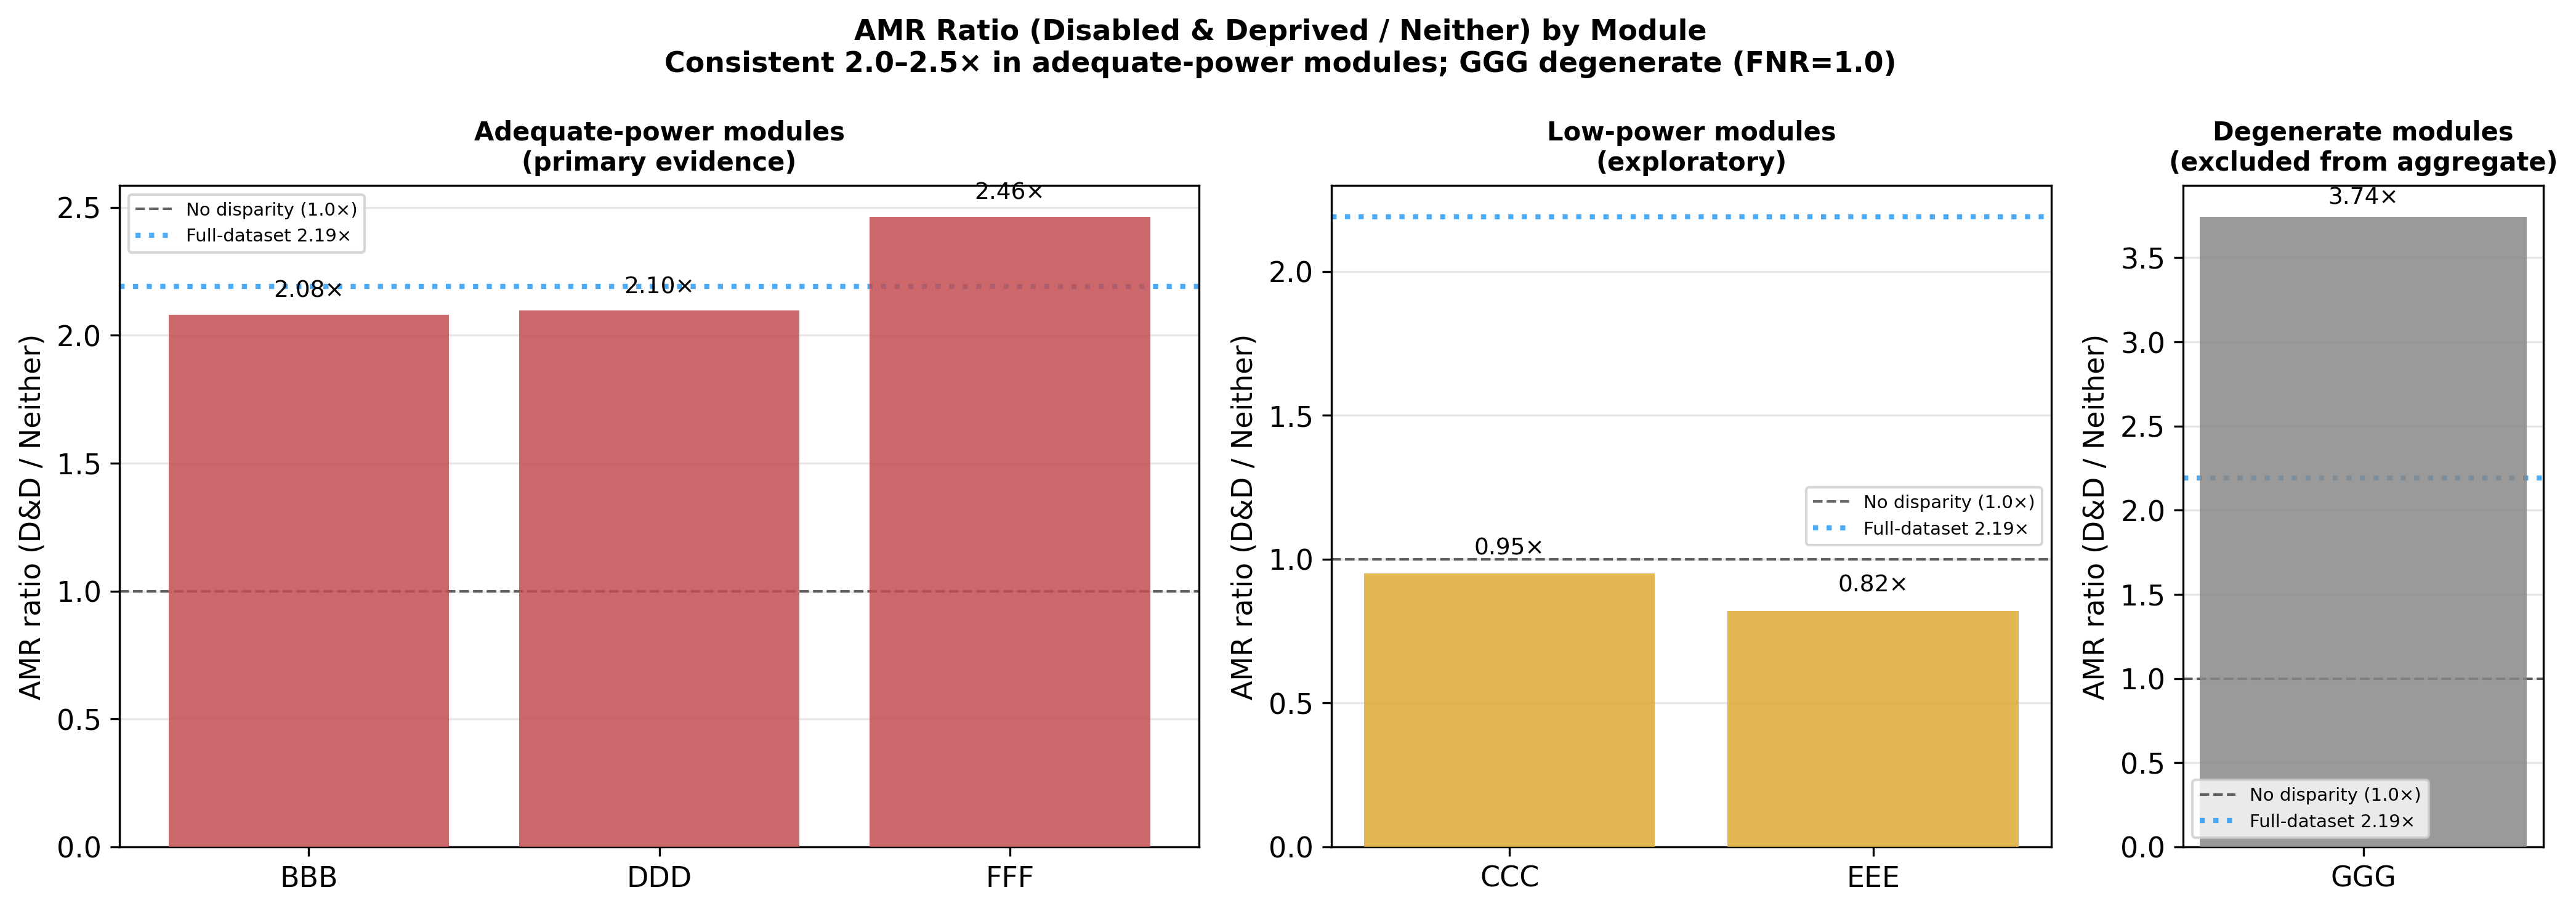
\includegraphics[width=0.95\textwidth]{fig_module_amr_ratios.png}
\caption{AMR ratio (D\&D / Neither) by module, stratified by evidence
quality. Left panel (adequate-power, primary evidence): all three modules
produce ratios of 2.08--2.46$\times$, closely bracketing the full-dataset
2.19$\times$ reference (blue dotted line). Centre panel (low-power,
exploratory): non-significant reversals consistent with small-sample variance.
Right panel (degenerate): GGG excluded from aggregate; ratio mechanically
inflated by FNR $= 1.0$.}
\label{fig:ratios}
\end{figure}

\subsubsection{Disability FNR Disparity: A Compositional Pooling Artefact}

The full-dataset disability FNR disparity (XGBoost: $\Delta = 0.057$,
$p = 0.043$) does not replicate in any of the six analysed modules (0/6
significant; 3/6 positive direction). A Spearman correlation between
per-module disability prevalence and per-module disability FNR disparity
yields $\rho = 0.43$ ($p = 0.40$), not significant but directionally
consistent with a compositional mechanism.

This pattern is consistent with a Simpson's-paradox-type artefact
\citep{simpson1951}: when modules with different disability compositions and
FNR profiles are pooled, a spurious aggregate signal emerges that reflects
composition rather than within-module discrimination. This is an important
methodological finding: aggregate fairness metrics computed over pooled
heterogeneous populations can misrepresent the nature and source of bias.
A university acting on an aggregate disability disparity without module-level
validation may target interventions at the wrong source. Module-level
validation, as conducted here, is a necessary component of a trustworthy
fairness audit \citep{gardner2018}.

Figure~\ref{fig:scatter} provides a further visualisation. The scatter of
withdrawal rate versus AMR disparity shows no systematic positive relationship
across modules, confirming the AMR finding is not simply driven by modules
with higher overall withdrawal rates.

\begin{figure}[ht]
\centering
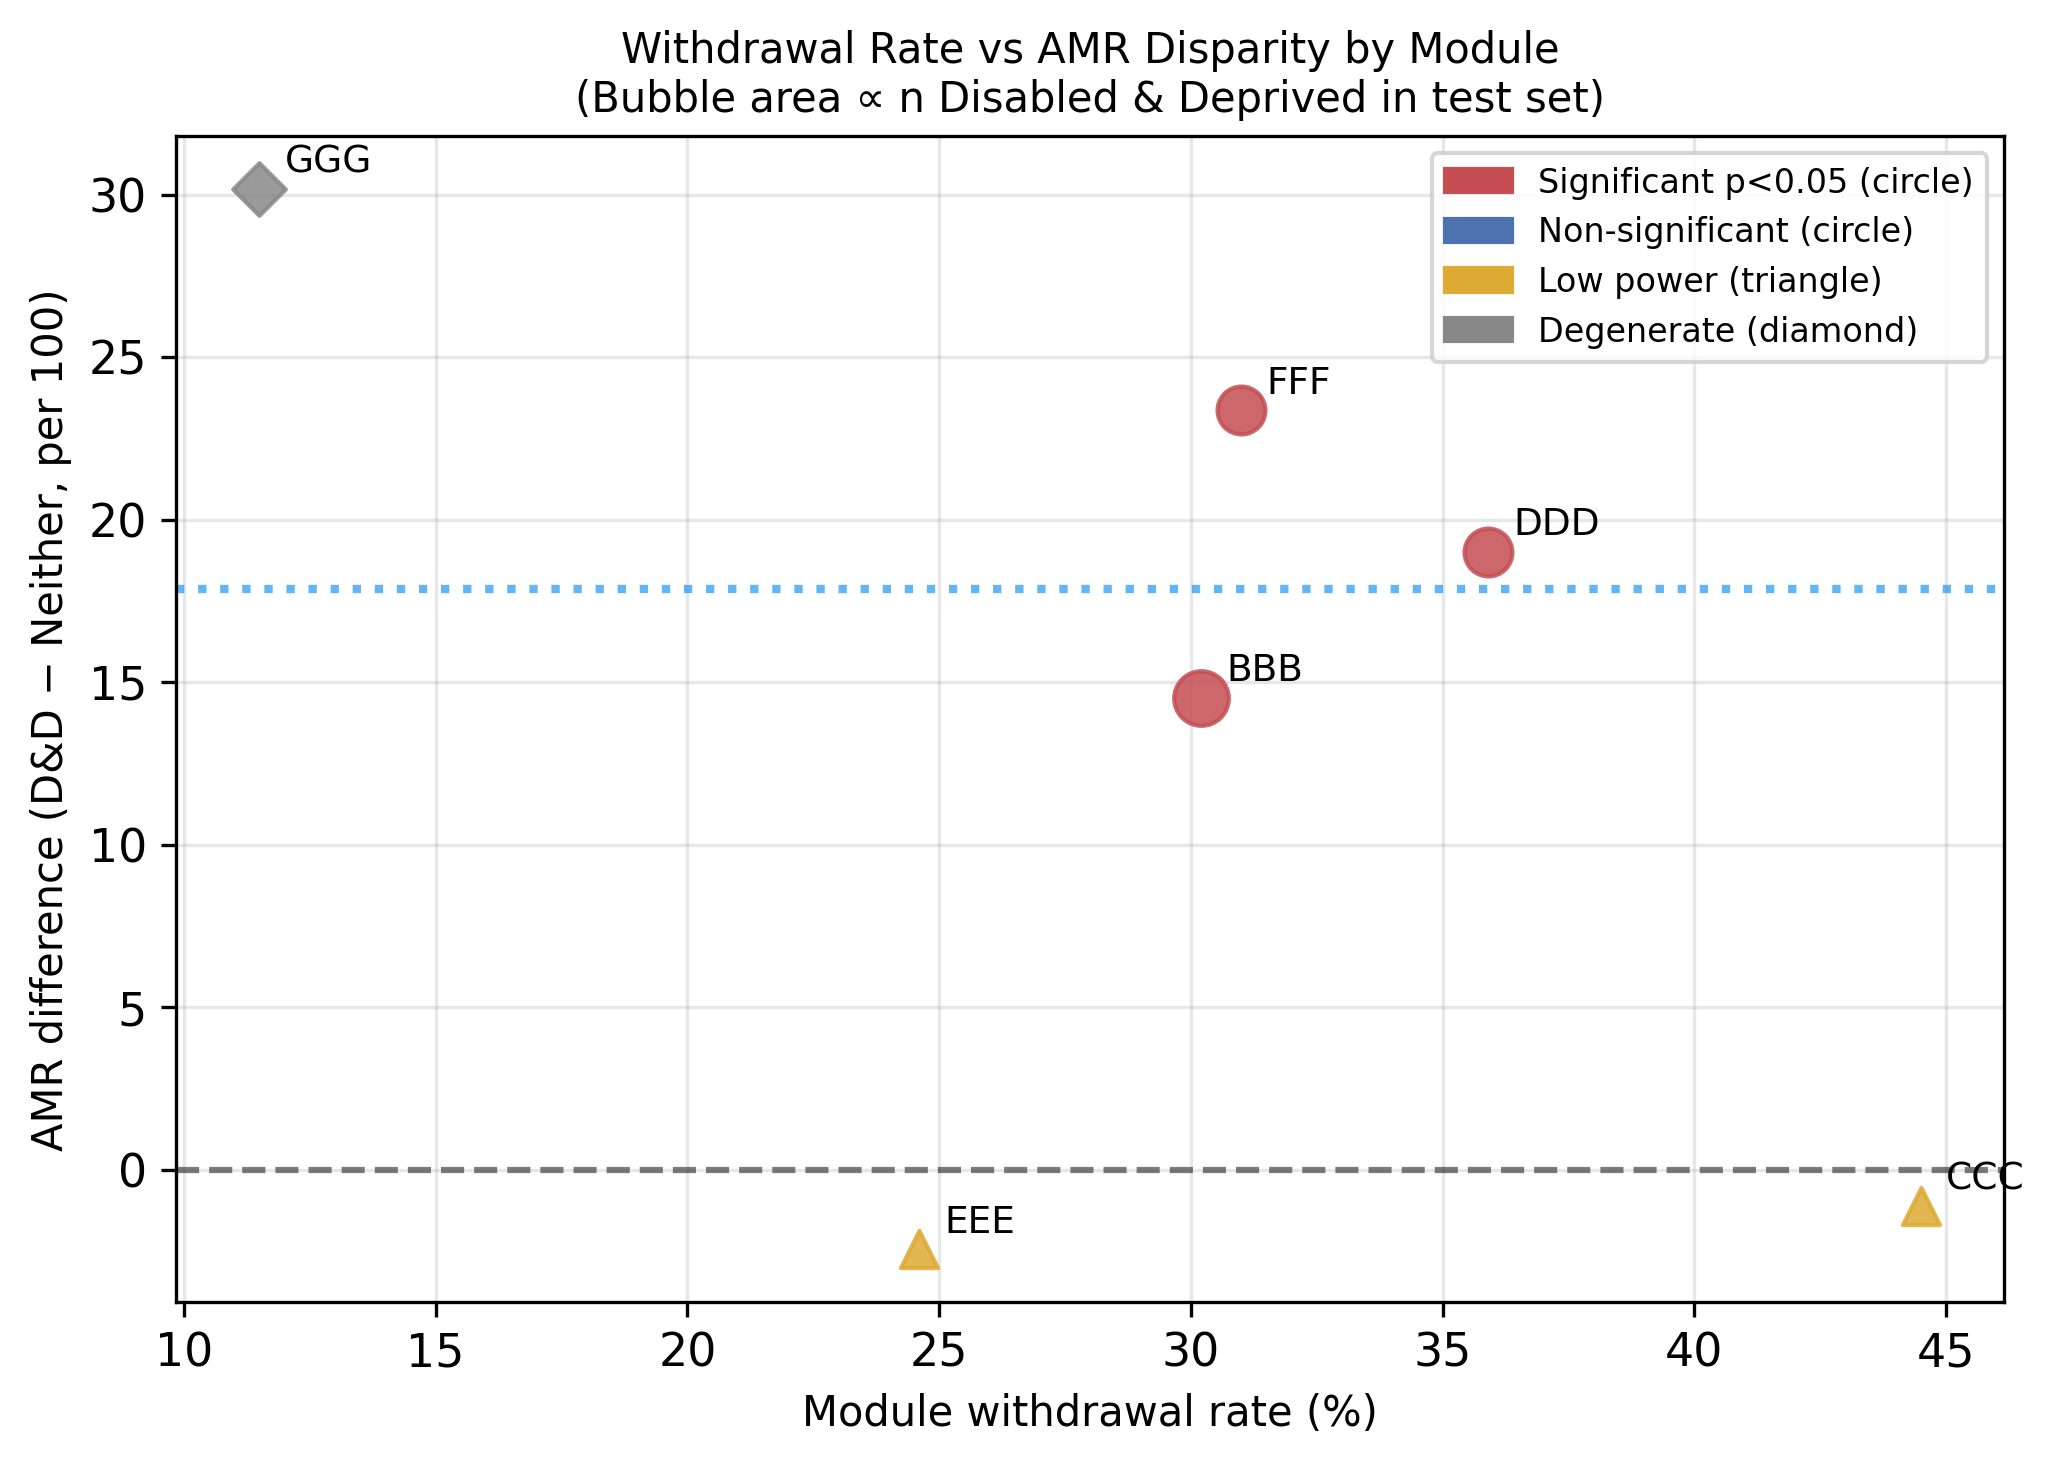
\includegraphics[width=0.75\textwidth]{fig_module_wr_scatter.png}
\caption{Module withdrawal rate versus AMR disparity. Bubble area
$\propto n$ Disabled \& Deprived in test set. The blue dotted line shows
the full-dataset AMR diff $= 17.88$. No systematic relationship between
withdrawal rate and AMR disparity is observed across modules ($\rho = 0.50$,
$p = 0.67$), indicating the AMR finding is not driven by overall module
difficulty.}
\label{fig:scatter}
\end{figure}

% -----------------------------------------------
% 5. DISCUSSION
% -----------------------------------------------
\section{Discussion}

\subsection{The Feature Leakage Problem in Learning Analytics Fairness Research}

The most consequential finding of this paper may be methodological. The
40-fold reduction in AUC when outcome-correlated features are excluded (from
0.995 to 0.805) indicates that a substantial portion of the predictive
performance reported in prior OULAD studies reflects models that have
inadvertently learned the outcome rather than early engagement patterns. This
is a specific instance of the leakage problem formalised by \citet{kaufman2012}.

The implication is direct: fairness conclusions from models trained on
assessment submission status, scores, or unregistration records may be
unreliable. The disparity patterns under leakage differ from those under
honest prediction because leaky features can correlate differently with
sensitive attributes than genuine engagement features do. The findings here
describe a more realistic deployment scenario: predicting withdrawal from
observable engagement behaviour at 28 days, not from administrative records
that become available only after withdrawal has begun.

\subsection{The AMR Metric: Absolute Harm in Operational Context}

The AMR metric makes the consequence of the impossibility theorem proved by
\citet{chouldechova2017} concrete. The D\&D group
has a 51.9\% withdrawal rate versus 27.5\% for the reference group. Even with
equal FNR, the absolute number of missed at-risk students per 100 enrolled
would be $51.9/27.5 \approx 1.89\times$ higher. The additional FNR disparity
amplifies this to 2.19$\times$. A university with 1,000 D\&D students enrolled
can expect the model to miss approximately 180 more at-risk individuals than
it would miss if those students had the reference group's base rate. The
consistency of this ratio across all five classifiers (2.06--2.29$\times$) and
across three independent module cohorts (pooled 18.27 [9.25, 27.30]) confirms
it is a structural property of this data, not a statistical artefact.

\subsection{Module-Level Replication and the Limits of Aggregate Metrics}

The module-level replication has two contributions. The positive finding ---
consistent AMR ratios (2.08--2.46$\times$) with no significant heterogeneity
--- substantially strengthens the evidence base. The negative finding ---
disability FNR disparity does not replicate within modules --- illustrates a
general methodological hazard: aggregate fairness metrics can reflect
between-group compositional differences rather than within-group prediction
bias \citep{gardner2018, simpson1951}. This extends the intersectionality
argument of \citet{crenshaw1989} from cross-attribute to cross-cohort analysis.

\subsection{Threshold Calibration as a Deployable Solution}

Strategy S1 achieves a 92\% FNR disparity reduction at a cost of 0.002 in F1
--- negligible for any practical deployment. Unlike in-processing mitigation,
this post-processing approach requires no retraining \citep{hardt2016}: a
university can apply group-specific thresholds to existing model probability
outputs without any infrastructure change. The failure of reweighting confirms
the theoretical prediction \citep{hardt2016} that in-processing interventions
are ineffective for groups as sparse as 3\% of the training set.

\subsection{UK Equality Act Implications}

The Equality Act 2010 \citep{equalityact2010} places positive duties on UK
universities to advance equality of opportunity. Standard VLE-based withdrawal
prediction systems systematically miss D\&D students at more than twice the
reference rate, even on a leak-free feature set. This arises from the
mathematical relationship between base rates, FNR, and absolute impact
\citep{chouldechova2017}, and can be corrected through post-processing
calibration with negligible accuracy cost. We encourage institutions to
include such calibration as standard practice in responsible AI governance
frameworks for learning analytics systems \citep{slade2013, prinsloo2013}.

% -----------------------------------------------
% 6. LIMITATIONS
% -----------------------------------------------
\section{Limitations}

\textbf{Feature set and AUC.} The leak-free feature set achieves
ROC-AUC $\approx 0.80$--$0.81$, below the 0.83--0.87 range in studies using
richer (but outcome-correlated) feature sets. This is an honest estimate.
Extending the feature set with genuinely pre-outcome features such as prior
academic records could improve performance without introducing leakage.

\textbf{Module-level replication power.} The module-level replication covers
three adequately-powered cohorts. The minimum detectable effect at 80\% power
is approximately 14--15 FNR percentage points; observed module effects
generally exceed this threshold. The Cochran $Q$ result ($I^2 = 0\%$)
strengthens confidence that the three estimates are consistent.
Multi-institution replication remains an important future priority.

\textbf{Intersectional group size.} The D\&D test group ($n = 185$,
$\approx 96$ positives) is adequate for the full-dataset bootstrap analysis
but produces wide individual module CIs (e.g.\ BBB: [1.5, 29.0]). The IVW
pooled estimate [9.25, 27.30] is tighter and preferred for summary reporting.

\textbf{Single dataset.} OULAD represents a non-traditional student
population (distance learning, Open University). Fairness profiles may differ
at campus-based universities with different demographic compositions.

\textbf{Threshold calibration and data protection.} Group-specific thresholds
require disability and deprivation status to be known at prediction time. UK
data protection law restricts certain uses of sensitive personal data;
institutions should seek legal advice before implementing group-specific
thresholds in production systems.

\textbf{AMR assumptions.} AMR uses the population base rate as the reference
for individual-level harm. Decision-theoretic refinements conditioning on
intervention-seeking behaviour may be more appropriate in contexts where
disadvantaged groups face barriers to accessing support even when identified.

% -----------------------------------------------
% 7. CONCLUSION
% -----------------------------------------------
\section{Conclusion}

This paper has made four contributions to the learning analytics fairness
literature.

First, we identified and corrected a systematic feature leakage problem in
OULAD fairness research \citep{kaufman2012}: including submission records and
unregistration dates inflates ROC-AUC from 0.805 to 0.995 and renders
fairness conclusions unreliable. Our leak-free feature set and associated code
assertions provide a methodological template for future work.

Second, we introduced the Absolute Miss Rate (AMR) metric and demonstrated
that D\&D students face a 2.19$\times$ AMR ratio ($\Delta = 17.88$ per 100,
CI: [11.02, 24.67], $p < 0.0001$; consistent across all five classifiers,
2.06--2.29$\times$). This is not visible under equalized-odds analysis because,
as \citet{chouldechova2017} proved, equal FNR is insufficient to equate
absolute harm when base rates differ.

Third, we provided the first module-level replication of an OULAD fairness
finding. The AMR ratio replicates in all three adequately-powered course
cohorts (2.08--2.46$\times$, all $p < 0.05$; IVW pooled 18.27 [9.25, 27.30],
$p = 0.0001$; $I^2 = 0\%$). The aggregate disability FNR disparity does not
replicate at module level --- a Simpson's-paradox-type compositional effect
\citep{simpson1951} that serves as a cautionary example for aggregate fairness
reporting.

Fourth, group-specific threshold calibration reduces FNR disparity by 92\%
(0.158 $\rightarrow$ 0.013) at a cost of 0.002 in system F1, requiring no
model retraining \citep{hardt2016} and immediately deployable in existing
university prediction pipelines.

These findings call for three changes in practice. Learning analytics
researchers should routinely audit features for outcome correlation
\citep{kaufman2012} before reporting fairness metrics. Universities deploying
withdrawal prediction should apply AMR alongside FNR and validate aggregate
findings at cohort level before acting on them \citep{gardner2018}. UK
institutions operating VLE-based prediction systems can apply group-specific
threshold calibration to existing model outputs, at negligible cost, to
substantially reduce the disproportionate miss rate for disabled students from
deprived backgrounds \citep{equalityact2010}. Code and processed features are
available at \url{https://github.com/valakhorasani/oulad-fairness}.

% -----------------------------------------------
% ACKNOWLEDGEMENTS
% -----------------------------------------------
\section*{Acknowledgements}

The author thanks the School of Computing and Mathematical Sciences at the
University of Leicester for support during this research.

\section*{Declaration of Conflicting Interests}

The author declares no conflicts of interest.

\section*{Funding}

This research received no specific funding from any agency in the public,
commercial, or not-for-profit sectors.

% -----------------------------------------------
% APPENDIX
% -----------------------------------------------
\appendix

\section{Module GGG: Raw AMR Values (Degenerate Case)}
\label{app:ggg}

Module GGG (wr $= 11.5\%$, $n_{\text{D\&D, test}} = 17$) is flagged as
degenerate: FNR$_{\text{D\&D}} = 1.000$ (the model never predicts withdrawal
for any D\&D student). This occurs because the very low module withdrawal rate
and small D\&D test group cause predicted probabilities to fall below 0.50 for
all D\&D students. The reported AMR$_{\text{D\&D}} = 41.20$ and AMR diff
$= 30.16$ are mechanically inflated and do not reflect a genuine fairness
signal. Values are reported here for transparency.

\begin{table}[ht]
\centering
\caption{Module GGG raw values (degenerate; excluded from aggregate).}
\label{tab:ggg}
\small
\begin{tabular}{lcccccc}
\toprule
Module & $n_{\text{D\&D, test}}$ & wr & AUC & FNR$_{\text{D\&D}}$ &
AMR$_{\text{D\&D}}$ & AMR diff \\
\midrule
GGG & 17 & 11.5\% & 0.690 & 1.000 & 41.20 & 30.16 \\
\bottomrule
\end{tabular}
\end{table}

\section{Low-Power Module Results}
\label{app:lowpower}

\begin{table}[ht]
\centering
\caption{Low-power module results. Directionally informative only; group
sizes are insufficient for reliable FNR estimation.}
\label{tab:lowpower}
\small
\begin{tabular}{lccccccc}
\toprule
Module & $n_{\text{D\&D}}$ & FNR$_{\text{D\&D}}$ & FNR$_{\text{Neither}}$ &
AMR$_{\text{D\&D}}$ & AMR diff & Ratio & $p$ \\
\midrule
CCC & 14 & 0.300 & 0.545 & 21.42 & $-1.12$ & 0.95$\times$ & 0.575 \\
EEE &  9 & 0.500 & 0.583 & 11.10 & $-2.44$ & 0.82$\times$ & 0.562 \\
\bottomrule
\end{tabular}
\end{table}

The reversals in CCC and EEE are non-significant and consistent with expected
sampling variance at $n_{\text{D\&D}} = 9$--$14$. They should not be
interpreted as evidence of protective bias.

% -----------------------------------------------
% REFERENCES
% -----------------------------------------------
\bibliographystyle{plainnat}
\bibliography{references}

\end{document}
